% Options for packages loaded elsewhere
\PassOptionsToPackage{unicode}{hyperref}
\PassOptionsToPackage{hyphens}{url}
%


\PassOptionsToPackage{table}{xcolor}

\documentclass[
  10pt,
  letterpaper,
]{article}

\usepackage{amsmath,amssymb}
\usepackage{iftex}
\ifPDFTeX
  \usepackage[T1]{fontenc}
  \usepackage[utf8]{inputenc}
  \usepackage{textcomp} % provide euro and other symbols
\else % if luatex or xetex
  \usepackage{unicode-math}
  \defaultfontfeatures{Scale=MatchLowercase}
  \defaultfontfeatures[\rmfamily]{Ligatures=TeX,Scale=1}
\fi
\usepackage{lmodern}
\ifPDFTeX\else  
    % xetex/luatex font selection
\fi
% Use upquote if available, for straight quotes in verbatim environments
\IfFileExists{upquote.sty}{\usepackage{upquote}}{}
\IfFileExists{microtype.sty}{% use microtype if available
  \usepackage[]{microtype}
  \UseMicrotypeSet[protrusion]{basicmath} % disable protrusion for tt fonts
}{}
\makeatletter
\@ifundefined{KOMAClassName}{% if non-KOMA class
  \IfFileExists{parskip.sty}{%
    \usepackage{parskip}
  }{% else
    \setlength{\parindent}{0pt}
    \setlength{\parskip}{6pt plus 2pt minus 1pt}}
}{% if KOMA class
  \KOMAoptions{parskip=half}}
\makeatother
\usepackage{xcolor}
\usepackage[top=0.85in,left=2.75in,footskip=0.75in]{geometry}
\setlength{\emergencystretch}{3em} % prevent overfull lines
\setcounter{secnumdepth}{-\maxdimen} % remove section numbering


\providecommand{\tightlist}{%
  \setlength{\itemsep}{0pt}\setlength{\parskip}{0pt}}\usepackage{longtable,booktabs,array}
\usepackage{calc} % for calculating minipage widths
% Correct order of tables after \paragraph or \subparagraph
\usepackage{etoolbox}
\makeatletter
\patchcmd\longtable{\par}{\if@noskipsec\mbox{}\fi\par}{}{}
\makeatother
% Allow footnotes in longtable head/foot
\IfFileExists{footnotehyper.sty}{\usepackage{footnotehyper}}{\usepackage{footnote}}
\makesavenoteenv{longtable}
\usepackage{graphicx}
\makeatletter
\def\maxwidth{\ifdim\Gin@nat@width>\linewidth\linewidth\else\Gin@nat@width\fi}
\def\maxheight{\ifdim\Gin@nat@height>\textheight\textheight\else\Gin@nat@height\fi}
\makeatother
% Scale images if necessary, so that they will not overflow the page
% margins by default, and it is still possible to overwrite the defaults
% using explicit options in \includegraphics[width, height, ...]{}
\setkeys{Gin}{width=\maxwidth,height=\maxheight,keepaspectratio}
% Set default figure placement to htbp
\makeatletter
\def\fps@figure{htbp}
\makeatother

% Use adjustwidth environment to exceed column width (see example table in text)
\usepackage{changepage}

% marvosym package for additional characters
\usepackage{marvosym}

% cite package, to clean up citations in the main text. Do not remove.
% Using natbib instead
% \usepackage{cite}

% Use nameref to cite supporting information files (see Supporting Information section for more info)
\usepackage{nameref,hyperref}

% line numbers
\usepackage[right]{lineno}

% ligatures disabled
\usepackage{microtype}
\DisableLigatures[f]{encoding = *, family = * }

% create "+" rule type for thick vertical lines
\newcolumntype{+}{!{\vrule width 2pt}}

% create \thickcline for thick horizontal lines of variable length
\newlength\savedwidth
\newcommand\thickcline[1]{%
  \noalign{\global\savedwidth\arrayrulewidth\global\arrayrulewidth 2pt}%
  \cline{#1}%
  \noalign{\vskip\arrayrulewidth}%
  \noalign{\global\arrayrulewidth\savedwidth}%
}

% \thickhline command for thick horizontal lines that span the table
\newcommand\thickhline{\noalign{\global\savedwidth\arrayrulewidth\global\arrayrulewidth 2pt}%
\hline
\noalign{\global\arrayrulewidth\savedwidth}}

% Text layout
\raggedright
\setlength{\parindent}{0.5cm}
\textwidth 5.25in 
\textheight 8.75in

% Bold the 'Figure #' in the caption and separate it from the title/caption with a period
% Captions will be left justified
\usepackage[aboveskip=1pt,labelfont=bf,labelsep=period,justification=raggedright,singlelinecheck=off]{caption}
\renewcommand{\figurename}{Fig}

% Remove brackets from numbering in List of References
\makeatletter
\renewcommand{\@biblabel}[1]{\quad#1.}
\makeatother

% Header and Footer with logo
\usepackage{lastpage,fancyhdr}
\usepackage{epstopdf}
%\pagestyle{myheadings}
\pagestyle{fancy}
\fancyhf{}
%\setlength{\headheight}{27.023pt}
%\lhead{\includegraphics[width=2.0in]{PLOS-submission.eps}}
\rfoot{\thepage/\pageref{LastPage}}
\renewcommand{\headrulewidth}{0pt}
\renewcommand{\footrule}{\hrule height 2pt \vspace{2mm}}
\fancyheadoffset[L]{2.25in}
\fancyfootoffset[L]{2.25in}
\lfoot{\today}
\makeatletter
\@ifpackageloaded{caption}{}{\usepackage{caption}}
\AtBeginDocument{%
\ifdefined\contentsname
  \renewcommand*\contentsname{Table of contents}
\else
  \newcommand\contentsname{Table of contents}
\fi
\ifdefined\listfigurename
  \renewcommand*\listfigurename{List of Figures}
\else
  \newcommand\listfigurename{List of Figures}
\fi
\ifdefined\listtablename
  \renewcommand*\listtablename{List of Tables}
\else
  \newcommand\listtablename{List of Tables}
\fi
\ifdefined\figurename
  \renewcommand*\figurename{Figure}
\else
  \newcommand\figurename{Figure}
\fi
\ifdefined\tablename
  \renewcommand*\tablename{Table}
\else
  \newcommand\tablename{Table}
\fi
}
\@ifpackageloaded{float}{}{\usepackage{float}}
\floatstyle{ruled}
\@ifundefined{c@chapter}{\newfloat{codelisting}{h}{lop}}{\newfloat{codelisting}{h}{lop}[chapter]}
\floatname{codelisting}{Listing}
\newcommand*\listoflistings{\listof{codelisting}{List of Listings}}
\makeatother
\makeatletter
\makeatother
\makeatletter
\@ifpackageloaded{caption}{}{\usepackage{caption}}
\@ifpackageloaded{subcaption}{}{\usepackage{subcaption}}
\makeatother
\ifLuaTeX
  \usepackage{selnolig}  % disable illegal ligatures
\fi
\usepackage[numbers,square,comma]{natbib}
\bibliographystyle{plos2015}
\usepackage{bookmark}

\IfFileExists{xurl.sty}{\usepackage{xurl}}{} % add URL line breaks if available
\urlstyle{same} % disable monospaced font for URLs
\hypersetup{
  pdftitle={Biomarker Infeksi Bakteri pada Febrile Neutropenia},
  hidelinks,
  pdfcreator={LaTeX via pandoc}}



\begin{document}
\vspace*{0.2in}

% Title must be 250 characters or less.
\begin{flushleft}
{\Large
\textbf\newline{Biomarker Infeksi Bakteri pada Febrile
Neutropenia} % Please use "sentence case" for title and headings (capitalize only the first word in a title (or heading), the first word in a subtitle (or subheading), and any proper nouns).
}
\newline
\\
% Insert author names, affiliations and corresponding author email (do not include titles, positions, or degrees).
dr. Kadek Adit Wiryadana\textsuperscript{1*}, dr. Ngakan Wira Suastika,
SpPD, K-HOM\textsuperscript{1*}
\\
\bigskip
\textbf{1} Universitas Udayana, 
\bigskip

% Insert additional author notes using the symbols described below. Insert symbol callouts after author names as necessary.
% 
% Remove or comment out the author notes below if they aren't used.
%
% Primary Equal Contribution Note
\Yinyang These authors contributed equally to this work.

% Additional Equal Contribution Note
% Also use this double-dagger symbol for special authorship notes, such as senior authorship.
%\ddag These authors also contributed equally to this work.

% Current address notes
\textcurrency Current Address: Dept/Program/Center, Institution Name, City, State, Country % change symbol to "\textcurrency a" if more than one current address note
% \textcurrency b Insert second current address 
% \textcurrency c Insert third current address

% Deceased author note
\dag Deceased

% Group/Consortium Author Note
\textpilcrow Membership list can be found in the Acknowledgments section.

% Use the asterisk to denote corresponding authorship and provide email address in note below.
* 
* 

\end{flushleft}



\linenumbers
\subsection{Abstrak}\label{abstrak}

\subsection{Pendahuluan}\label{pendahuluan}

Terdapat kemajuan besar dalam terapi pasien dengan penyakit keganasan
selama beberapa dekade terakhir dengan demikian mampu menurunkan angka
kematian akibat keganasan. Perkembangan ilmu dan teknologi telah
menghasilkan serangkaian agen kemoterapi baru dan modalitas pengobatan
modern lain yang telah berhasil diterapkan dalam praktik klinis,
termasuk transplantasi sumsum tulang dan sel punca. Namun sebagian besar
pilihan pengobatan ini membuka sebuah titik kelemahan yakni penekanan
terhadap imunitas. Neutropenia khususnya masih merupakan kelainan imun
yang paling signifikan akibat kemoterapi sehingga menyebabkan pasien
rentan terhadap infeksi. Meskipun terdapat peningkatan dalam
kelangsungan hidup jangka panjang, infeksi tetap menjadi komplikasi
utama dari terapi kegamasam dan menyebabkan sebagian besar kematian
terkait kemoterapi. Masalah ini akan dipersulit dengan dilema terkait
pemberian antibiotik dan pemilihannya yang tepat.\citep{sipsas}

Perkembangan terapi terkait febrile neutropenia pada dekade terakhir
cukup substansial.\citep{sipsas} Perkembangan pola agen infeksi serta
resistensi antibiotik memberikan tantangan khusus dalam mengembangkan
pedoman universal terkait febril neutropenia. Pada kasus febril
neutropenia, sampai saat ini dianut bahwa pemberian antibiotik sedini
mungkin merupakan pilar utama tatalaksana standar pada berbagai
institusi. Adanya perubahan tren resistensi bakteri menyebabkan
pemilihan antibiotik harus mengikuti pola kepekaan kuman lokal, sehingga
seharusnya pedoman pemilihan antibiotik harus menjadi perhatian penting
untuk diperbaharui secara berkala.\citep{sipsas}

Kecenderungan terapi bertumpu pada monoterapi antibiotik spektrum luas
generasi terbaru menggantikan pola terapi klasik dengan kombinasi
antibiotik. Pemberian monoterapi antibiotik secara empiris disisi lain
dapat meningkatkan risiko resistensi bakteri.\citep{sipsas} Selain itu,
febril neutropenia akibat agen infeksi non bakterial tentu akan
menempatkan pemberian antibiotik sebagai sesuatu yang tidak bermanfaat
bahkan cenderung merugikan. Solusi yang diperlukan adalah berupa
modalitas diagnostik yang cepat memberikan informasi terkait etiologi
febril neutropenia sehingga dapat membantu dalam mengambil keputusan
apakah pemberian antibiotik dapat menjadi sesuatu yang bermanfaat.

\subsection{Febril Neutropenia}\label{febril-neutropenia}

Kemoterapi sitotoksik klasik dan radioterapi sebagian besar memediasi
efek antineoplastiknya melalui pengaruh replikasi DNA. Salah satu
komplikasi dari supesi replikasi DNA adalah penurnan jumlah sel, salah
satunya adalah keadaan neutropenia. Demam Neutropenia/ Febrile
Neutropenia (FN) adalah kondisi yang berpotensi mengancam nyawan yang
didefinisikan sebagai demam dengan suhu oral tunggal ≥38.3 °C (101 °F)
atau suhu ≥38.0 °C (100.4 °F) yang dipertahankan selama periode 1 jam,
dikombinasikan dengan neutropenia berat yang didefinisikan sebagai
jumlah neutrofil absolut (ANC) \textless500 sel/mm\textsuperscript{3}
atau ANC yang diperkirakan menurun hingga \textless500
sel/mm\textsuperscript{3} selama 48 jam berikutnya.\citep{Zimmer2019} FN
merupakan komplikasi pada hampir 50\% pasien dengan tumor padat dan pada
\textgreater80\% pasien dengan keganasan hematologi yang menjalani
kemoterapi atau setelah transplantasi sel induk hematopoietik (HSCT) dan
paling sering terjadi sebagai akibat dari translokasi bakteri usus
disertai tidak adanya antimikrobiosis langsung yang mediasi oleh
neutrofil dan rendahnya respons efektor sistem imun. Faktor risiko FN
termasuk ANC \textless100 sel/mm\textsuperscript{3} selama \textgreater7
hari, usia lebih tua, \emph{performance} status buruk, adanya kondisi
komorbiditas, dan penyakit stadium lanjut.\citep{baluch2019infections}
FN dianggap sebagai keadaan darurat medis, dengan angka kematian
keseluruhan sebesar 5\% hingga 20\%, dan dapat meningkat hingga 50\%
pada pasien yang mengalami syok.\citep{carmona-bayonas2015}

Dengan tidak adanya penjelasan alternatif, dokter harus berasumsi bahwa
demam pada pasien dengan neutropenia akibat terapi kanker adalah akibat
dari infeksi. Pendekatan diagnostik awal harus memaksimalkan peluang
untuk menegakkan diagnosis klinis dan mikrobiologis yang dapat
mempengaruhi pilihan dan prognosis antibakteri.\citep{taplitz2018}

\subsection{Biomarker Infeksi Bakteri}\label{biomarker-infeksi-bakteri}

Terdapat variasi yang luas pada patogen yang ditemukan terlibat dalam
proses febril neutropenia. Hal ini salah satunya dijelaskan karena
sumber utama patogen pada kondisi imunokompromised adalah flora endogen.
Namun, banyak mikroorganisme eksogen lain dengan virulensi rendah yang
dapat diperoleh dari udara atau air yang terkontaminasi atau dari kontak
dengan pasien, personel, atau peralatan lain dapat menjadi invasif dan
menyebabkan infeksi pada pasien dengan kondisi neutropenia. Secara
historis, basil gram negatif yang muncul dari saluran pencernaan telah
menjadi patogen utama pada inang neutropenia. Antara tahun 1960an hingga
pertengahan tahun 1970an,Escherichia coli, Klebsiella spesies, dan
Pseudomonas aeruginosa menyumbang sebagian besar infeksi yang
didokumentasikan secara mikrobiologis di sebagian besar pusat kanker.
Sejak diperkenalkannya beta-laktam spektrum luas, beberapa institusi di
Amerika Serikat dan Eropa telah mengalami penurunan bakteremia bakteri
batang gram negatif dan peningkatan infeksi akibat kokus gram
positif.\citep{sipsas}

\subsubsection{Biomarker Hematologi}\label{biomarker-hematologi}

\paragraph{Jumlah Leukosit}\label{jumlah-leukosit}

Saat terjadi infeksi bakteri, neutrofil dengan cepat direkrut ke fokus
infeksi dan menginisiasi respon imun, mengikat, dan mengfagositosis
mikroorganisme.\citep{bernardi2024} Sejumlah besar neutrofil dikonsumsi
di lokasi infeksi sehingga harus terus disuplai ke tempat yang
terinfeksi dari sumsum tulang melalui aliran darah.12 Oleh karena itu,
perubahan dinamis terjadi pada jumlah leukosit (WBC) dan neutrofil (ANC)
yang mungkin terjadi mencerminkan kondisi real-time pasien dengan
infeksi bakteri. Namun, belakangan ini tinjauan sistematis dan
meta-analisis studi diagnostik menunjukkan bahwa sel darah putih
memberikan sensitivitas(58\%) dan spesifisitas 73\% rendah, atau lebih
rendah jika dibandingkan dengan prokalsitonin (PCT) dan \emph{C-reactive
protein} (CRP).\citep{Yo2012} Sebuah penelitian yang membandingkan WBC,
ANC, dan CRP sehubungan dengan timbulnya demam menemukan bahwa CRP
memiliki sensitivitas dan spesifisitasnya lebih baik dibandingkan WBC
atau ANC, tanpa memandang durasi demam. Menariknya, di penelitian ini
semua biomarker bekerja lebih baik dengan durasi demam \textgreater12
jam.\citep{pratt2007}

\paragraph{Indeks terkait trombosit}\label{indeks-terkait-trombosit}

Penelitian telah mengidentifikasi trombosit sebagai salah satu komponen
pertama dalam respons penyakit infeksi yang melibatkan proses
fagositosis patogen atas peran dari protein yang disimpan dalam granul
platelet. Indeks trombosit yang beragam, seperti PNLR/ \emph{platelet to
neutrophil-lymphocyte ratio} (rasio trombosit terhadap
neutrofil/limfosit), PNR/ \emph{platelet to neutrophil ratio} (rasio
trombosit terhadap neutrofil) dan protein yang disekresikan, seperti
sP-selectin, CXCL4, CXCL7, dan serotonin, telah dipelajari sebagai
penanda untuk membedakan infeksi virus dan bakteri.\citep{semple2011}
Mengingat pasien yang datang ke UGD dengan demam dini (\textless12 jam),
nilai PNLR lebih tinggi telah diamati pada mereka yang menderita infeksi
bakteri.\citep{vassiliou2014a} Molekul lain yang ditemukan pada platelet
dan dapat menjadi penanda infeksi bakteri adalah CXCL7 dan sP-selectin.
Kedua marker tersebut baik secara tungga dan digabungkan, secara
statistik signifikan untuk membedakan sepsis dan infeksi bakteri dari
penyebab lain.\citep{zonneveld2014} CXCL4 memiliki peran dalam respon
imun terhadap virus, dan peningkatannya dalam aliran darah tidak
signifikan pada pasien dengan infeksi bakteri. Namun nilai-nilai
tersebut belum terstandarisasi dan penelitian lebih lanjut diperlukan
untuk memastikan nilai normal pada populasi sehat dan dalam kondisi
klinis yang beragam.\citep{heijnen2015}

\subsubsection{Biomarker Inflamasi}\label{biomarker-inflamasi}

\paragraph{C-Reactive protein}\label{c-reactive-protein}

C-reactive Protein (CRP) saat ini menjadi marker inflamasi yang paling
banyak diperiksa. CRP merupakan molekul yang disintesis oleh liver
setelah mendapatkan stimulasi sitokin (IL-1 Beta, IL-6 dan TNF-Alpha)
dalam waktu 4-6 jam setelah terjadi kerusakan jaringan. Kadar CRP dalam
darah akan mencapai puncak dalam 36-50 jam paska stimulasi sitokin
terkait sehingga nilai CRP harus diinterpretasikan dengan hati-hati
ketika demam terjadi \textless12 jam. CRP merupakan salah satu komponen
yang berperan dalam imunitas fubuh melalui aktivasi komplemen melalui
jalur klasik, modulasi aktivitas fagositik sel dan meningkatkan
\emph{cell-mediated cytotoxicity}.\citep{bernardi2024}

Peningkatan kadar CRP dapat disebabkan oleh kondisi selain infeksi,
misalnya trauma, keganasan, gangguan rematologi, luka bakar dan
pankreatitis sehingga nilai CRP harus diinterpretasikan dengan hati-hati
dalam kasus ini.\citep{pepys2003} Sebaliknya, penurunan atau supresi
kadar CRP dapat terjadi pada kondisi gagal hati (\emph{liver failure})
dan imunokompromais.\citep{dyer2018} Namun demikian, beberapa penelitian
menunjukkan kegunaan CRP untuk identifikasi dini demam yang merupakan
akibat dari infeksi bakteri.\citep{verbakel2017} Dilema krusial dalam
praktik klinis adalah ambang batas yang digunakan untuk identifikasi
infeksi bakteri. Nilai batas yang sangat rendah akan menjadi sangat
sensitif namun kurang spesifik, dan nilai batas yang sangat tinggi akan
bersifat spesifik namun kurang sensitif. Dalam penelitian terbaru pada
populasi pediatri yang dilakukan oleh Verbakel dkk., nilai batas 75 mg/L
dapat digunakan sebagai ambang nilai CRP untuk menentukan pasien yang
memiliki risiko lebih besar mengalami infeksi bakteri berat dan batas
CRP sebesar 20 mg/L mengidentifikasi anak-anak yang berisiko rendah.

\paragraph{Procalcitonin}\label{procalcitonin}

Prokalsitonin (PCT) adalah prekursor protein asam amino untuk kalsitonin
yang diproduksi oleh sel parafollicular. Pada kondisi normal, kadar PCT
serum lebih rendah dari 0,05 ng/mL, sedangkan pada infeksi bakteri dapat
meningkat hingga 700 ng/L. Selama infeksi bakteri, tempat produksi PCT
tidak terbatas pada sel neuroendokrin. Pelepasan PCT diinduksi dengan
meningkatkan ekspresi gen CALC1 pada sel di seluruh tubuh, dipicu oleh
endotoksin atau faktor humoral, yaitu IL-1, TNF-alfa, dan IL-6.
Konsentrasi PCT meningkat lebih cepat dibandingkan kadar CRP pada pasien
SBI. Kadar PCT mulai meningkat pada 2 jam sejak awal infeksi dan
mencapai puncak serum pada 24 hingga 36 jam oleh karena itu PCT telah
terbukti menjadi biomarker yang lebih unggul dibandingkan dengan CRP
untuk mendeteksi infeksi bakteri di
UGD.\citep{Principi2017, bernardi2024}

\paragraph{Cytokines dan Chemokines}\label{cytokines-dan-chemokines}

Interaksi reseptor mirip Tol (TLR) yang terletak di permukaan membran­
permukaan sel penyaji antigen (APC) dan monosit dengan kelompok
\emph{pattern recognition receptor} (PAMPs) menghasilkan inisiasi
kaskade pensinyalan dan ekspresi gen yang terlibat dalam peradangan,
imunitas adaptif, dan metabolisme sel. Hal ini menyebabkan ekspresi gen
yang disebut ``\emph{early activation genes}'' dan pelepasan sitokin
(misalnya IFN- γ , IL-1, IL-6, IL-8, IL-12) serta komponen komplemen dan
koagulasi.\citep{Jarczak2021} Peningkatan sitokin pro dan anti-inflamasi
secara sistemik pada fase awal dianggap sebagai ciri klasik proses
infeksi bakteri. Sitokin dan kemokin telah dianggap sebagai biomarker
infeksi bakteri yang menjanjikan karena keterlibatan awal dalam respon
imun tubuh terhadap infeksi, terutama dalam beberapa tahun terakhir
berkat adanya kemajuan dalam teknis pendeteksian sitokin dan kemokin
dalam sampel darah. Selain itu, produksi CRP dan PCT bergantung pada
pelepasan sitokin, diperkirakan bahwa pengukuran sitokin dapat
memberikan evaluasi perkembangan sepsis yang lebih awal dan lebih
efektif dibandingkan dengan biomarker yang digunakan secara
tradisional.\citep{Boscarino2023}

Salah satu sitokin yang banyak diteliti adalah IL-6 terutama dalam
perannya pada infamasi sistemik. Hal Ini digambarkan sebagai sitokin
pro-inflamasi fase akut, yang meningkatkan kadarnya dalam darah selama
rentang waktu 6 jam pertama selama infeksi bakteri. Onset ini lebih awal
dari peningkatan CRP.\citep{Barichello2022, Biron2015}

Peran penting peningkatan kadar IL-10 dalam respons anti-inflamasi
ditemukan menjadi prediktor luaran yang lebih buruk pada pasien
neutropenia paska kemoterapi dengan sepsis. Pada temuan terbaru, IL-10
muncul dengan spesifisitas tinggi dan sensitivitas sedang. Walaupun IL-6
menurun dengan cepat dalam 12 jam pertama sejak timbulnya infeksi pada
darah, IL-10 cenderung bertahan lebih lama selama keadaan
septik.\citep{bernardi2024}

Peran diagnostik dari biomarker secara tunggal telah banyak diteliti,
namun banyak penulis menyatakan keunggulan kombinasi biomarker darah
dibandingkan tes individual dalam diagnosis banding etiologi
infeksi.\citep{theodosiou2019, tamelyte2019} Kombinasi WBC, ANC, CRP,
IL-2, dan IL-6 meningkatkan sensitivitas hingga 96\%, spesifisitas 81\%,
dan besar AUC 0,942 (CI 95\%, 0,859 hingga 0984) dalam menentukan
infeksi akibat bakteri dibandingkan yang etiologi lain.\citep{zeng2022}
Demikian pula, dengan mencocokkan CRP dengan kadar IL-10 diperoleh nilai
diagnostik yang lebih tinggi dalam menentikan etiologi bakteri
(spesifisitas dari 77\% menjadi 98\%, sensitivitas
75\%.\citep{bernardi2024}

Studi pendahuluan belakangan ini menunjukkan hasil yang baik mengenai
spesifisitas IL-27 dalam prediksi awal infeksi bakteri pada pasien
kondisi sakit kritis. Dengan menggunakan database ekspresi genom
anak-anak kritis di UGD pediatrik, gen prediktor yang mengkode protein
IL-27 dijelaskan; khususnya, EB13 (subunit dari IL-27), tampaknya
memiliki peran prediktif yang tinggi terhadap infeksi bakteri (lebih
dari 90\%). Dibandingkan dengan PCT, IL-27 berkinerja lebih baik dalam
membedakan infeksi bakteri dan virus. Temuan ini, meskipun masih awal,
mengarah pada pertimbangan IL-27 sebagai biomarker yang efektif dalam
sepsis bakterial, menunjukkan spesifisitas 95\% dalam mendeteksi
infeksi.\citep{Hanna2015, Wong2012a}

\subparagraph{Interleukines}\label{interleukines}

Van Houten dkk. menemukan bahwa dengan pengujian yang menggabungkan tiga
biomarker, yaitu TRAIL, IP-10, dan CRP, dapat membedakan infeksi bakteri
dan virus pada pasien demam dengan sensitivitas 86,7\% dan spesifisitas
91,1\%.\citep{van2017} Dalam penelitian berbasis proteomik yang berfokus
pada respon imun inang, menunjukkan bahwa kombinasi ketiga biomarker ini
menunjukkan parameter diagnostik yang lebih baik dibandingkan dengan
kombinasi biomarker inflamasi rutin pada pasien yang menderita demam
dengan dengan etiologi belum diketahui. Papan et al., dalam studi kohort
prospektif multinasional, memvalidasi kinerja diagnostik dari TRAIL,
IP-10, dan CRP dalam kohort luas pasien anak dengan infeksi saluran
pernafasan atau demam tanpa etiologi yang diketahui, menunjukkan
kemampuannya untuk mendukung diagnosis etiologi virus dan mengurangi
resep antibiotik.\citep{Papan2022} Interaksi antara CRP, IP-10 dan TRAIL
diilustrasikan pada Fig~\ref{fig-CRPIP10TRAIL}

\begin{figure}

\centering{

\href{https://www.mdpi.com/2218-273X/14/1/97}{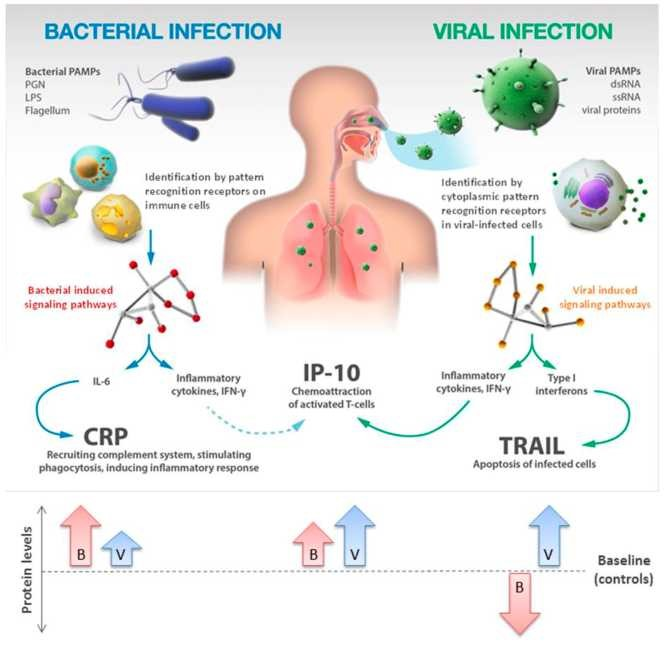
\includegraphics{image/infection_viralvsbacterial.jpg}}

}

\caption{\label{fig-CRPIP10TRAIL}Interact CRP, IP-10 dan TRAIL sebagai
marker infeksi}

\end{figure}%

\subparagraph{Trail}\label{trail}

\emph{Tumor necrosis factor-related apoptosis-inducing ligand} (TRAIL)
adalah protein transmembran tipe II yang termasuk dalam superfamili TNF
terlibat dalam regulasi respon imun bawaan dan
adaptif.\citep{Gyurkovska2016} TRAIL terlibat dalam sepsis dengan
menginduksi apoptosis sel inflamasi dan menurunkan regulasi inflamasi.
Banyak peneliti telah mengeksplorasi hubungan antara kadar TRAIL
terlarut (sTRAIL) pada pasien septik dan risiko kematian dan menemukan
bahwa tingkat sTRAIL yang rendah tampaknya dikaitkan dengan risiko
kematian yang tinggi, dengan pasien yang sintas memiliki tingkat sTRAIL
yang jauh lebih
tinggi.\citep{Papan2023, Fröhlich2023, Ashkenazi-Hoffnung2018}

\subparagraph{IP-10}\label{ip-10}

IP-10 (\emph{Interferon-gamma-inducible protein 10}) adalah kemokin yang
diekspresikan oleh sel penyaji antigen sebagai respons terhadap IFN- γ
dan menarik sel T yang teraktivasi ke fokus
peradangan.\citep{Ashkenazi-Hoffnung2021} Biomarker ini berperan dalam
respon terhadap infeksi bakteri, khususnya dalam diagnosis dan
penatalaksanaan infeksi saluran kemih, TBC, dan penyakit
autoimun.\citep{van2017}

\subsubsection{Molekul Adhesi Sel}\label{molekul-adhesi-sel}

Beberapa molekul adhesi sel, termasuk presepsin, molekul diferensiasi
cluster-64 (CD64), \emph{soluble trigger receptor expressed on myeloid
cell-1} (sTREM1), dan pentraxin3, untuk sementara digunakan untuk
membedakan pasien sepsis dan non-septik.

\paragraph{Presepin}\label{presepin}

Presepsin (sCD14-ST) adalah protein yang terkait dengan pembelahan sel
CD14, suatu bentuk reseptor lipopolisakarida (LPS) yang larut, yang
mengenali pola molekuler terkait patogen (PAMP) dan memicu respons imun
bawaan.\citep{Velissaris2021, Kyriazopoulou2023} Ini menjelaskan
peningkatan kadarnya menjadi spesifik pada infeksi bakteri, di mana
mekanisme patogenetik yang mendasarinya diekspresikan melalui aksi LPS.

Presepsin tampaknya memiliki spesifisitas dan sensitivitas yang baik
pada sepsis dan berkorelasi dengan mortalitas di rumah sakit pada pasien
dengan sepsis dan syok septik, dengan potensi diagnostik yang dapat
meningkat jika digabungkan dengan parameter klinis. Selama keadaan
infeksi bakteri, konsentrasi nilai absolut meningkat dalam waktu 2 jam.
Presepsin adalah satu-satunya biomarker yang jika tetap meningkat pada
pasien dengan infeksi barkteri hal ini dapat dikaitkan dengan risiko
kematian yang lebih tinggi selama masa perawatan.\citep{Wu2017} Namun,
meskipun literatur mendukung peran potensialnya di UGD dan dalam
perawatan intensif, beberapa penelitian tidak menunjukkan keunggulan
presepsin dibandingkan dengan biomarker lain dalam hal sensitivitas dan
spesifisitas.\citep{Romualdo2014}

\paragraph{STREM-2}\label{strem-2}

\emph{Triggering receptor expressed on myeloid cells 1} (TREM-1) adalah
reseptor imun bawaan yang memainkan peran penting dalam amplifikasi
respon imun bawaan terhadap infeksi dengan menstimulasi pelepasan
sitokin pro-inflamasi.\citep{Smok2020} sTREM-1 dilepaskan dari
monosit/makrofag dan neutrofil selama aktivasi. Adanya infeksi bakteri
meningkatkan kadar sTREM-1. Bentuk larut dari reseptor ini, sTREM-1,
dilepaskan dari membran sel dan disekresi ke dalam sirkulasi selama
infeksi.\citep{Esposito2016, Balanza2020}

Tinjauan sistematis dan meta-analisis baru-baru ini mengevaluasi peran
potensial sTREM sebagai pendukung dalam diagnosis infeksi bakteri.
Namun, sensitivitas rendah dan spesifisitas sedang untuk sTREM-1 dalam
membedakan etiologi infeksi bakteri atau virus telah dilaporkan sehingga
mengurangi potensi manfaat klinisnya.\citep{Esposito2016}

\subsection{Pilihan Biomarker Infeksi Bakteri pada Febril
Neutropenia}\label{pilihan-biomarker-infeksi-bakteri-pada-febril-neutropenia}

Keterbatasan kecepatan dan sensitivitas kultur darah telah meciptakan
usaha untuk menemukan penanda biomarker inflamasi, seperti
\emph{C-reactive Protein}, interleukin-6 dan interleukin-8, dan
prokalsitonin, sebagai penanda potensial untuk memandu keputusan
penggunaan antimikroba.\citep{taplitz2018} Dalam pedoman IDSA tahun
2011, data pada saat itu tidak cukup untuk merekomendasikan penggunaan
rutin biomarker serum ini.\citep{Freifeld2011} Saat ini sudah terdapat
data dari tinjauan sistematis dengan metaanalisis yang melaporkan
perkiraan akurasi diagnostik untuk biomarker prokalsitonin untuk
diagnosis bakteremia.\citep{Hoeboer2015} Dalam analisis subkelompok
terhadap 320 pasien immunocompromised/neutropenic, area di bawah kurva
(AUC) adalah 0,71 untuk memprediksi bakteremia (AUC 0,70 hingga 0,80
dianggap sebagai tingkat akurasi diagnostik yang baik). Sensitivitasnya
adalah 66\% (95\% CI, 54\% hingga 76\%) dan spesifisitasnya adalah 78\%
(95\% CI ,71\% hingga 83\%), dengan tingkat heterogenitas statistik yang
tinggi (I2= 76\%). Sebuah studi tambahan menemukan bahwa
\emph{lipopolysaccharide-binding protein} (LBP) memiliki akurasi
diagnostik yang serupa dengan prokalsitonin atau IL-6 untuk diagnosis
infeksi.\citep{García2015} Pedoman terbaru dari \emph{American Society
of Clinical Oncology} (ASCO) menyimpulkan bahwa diperlukan lebih banyak
penelitian sebelum biomarker seperti prokalsitonin atau LBP dapat
direkomendasikan sebagai alat yang efektif untuk menentukan apakah
antibiotik harus dimulai.\citep{taplitz2018}

\subsection{Ringkasan}\label{ringkasan}

Respon inflamasi adalah mekanisme kompleks dimana banyak faktor biokimia
dan imunologi berkontribusi terhadap respon host pada infeksi bakteri.
Menyempurnakan biomarker dapat bermanfaat dalam penatagunaan antimikroba
sehingga peresepan dan dosis antibiotik lebih tepat. CRP dan
prokalsitonin masih merupakan biomarker yang paling banyak digunakan di
UGD untuk diagnosis infeksi bakteri. Sensitivitas keduanya meningkat
jika digabungkan sehingga masuk akal untuk mempertimbangkan keduanya
dalam evaluasi pasien dengan keluhan utama demam.


\nolinenumbers
  \bibliography{references.bib}

\end{document}
